\documentclass[dvipdfmx]{jsarticle}

\usepackage{graphicx}
\usepackage{wrapfig}
\usepackage{pgffor}
\usepackage{url}
\usepackage{todonotes}
\usepackage{cite}
\usepackage{xspace}
\usepackage{booktabs}
\usepackage{lscape}

\pagestyle{plain}

\newcommand{\Repeat}[2]{\foreach \x in {1,...,#1}{#2}}

\begin{document}
\begin{center}
\LARGE\bfseries これまでの研究実績概要
\end{center}

\section*{研究のスコープと専門性}

\begin{wrapfigure}{r}[0pt]{0.4\linewidth}
 \centering
 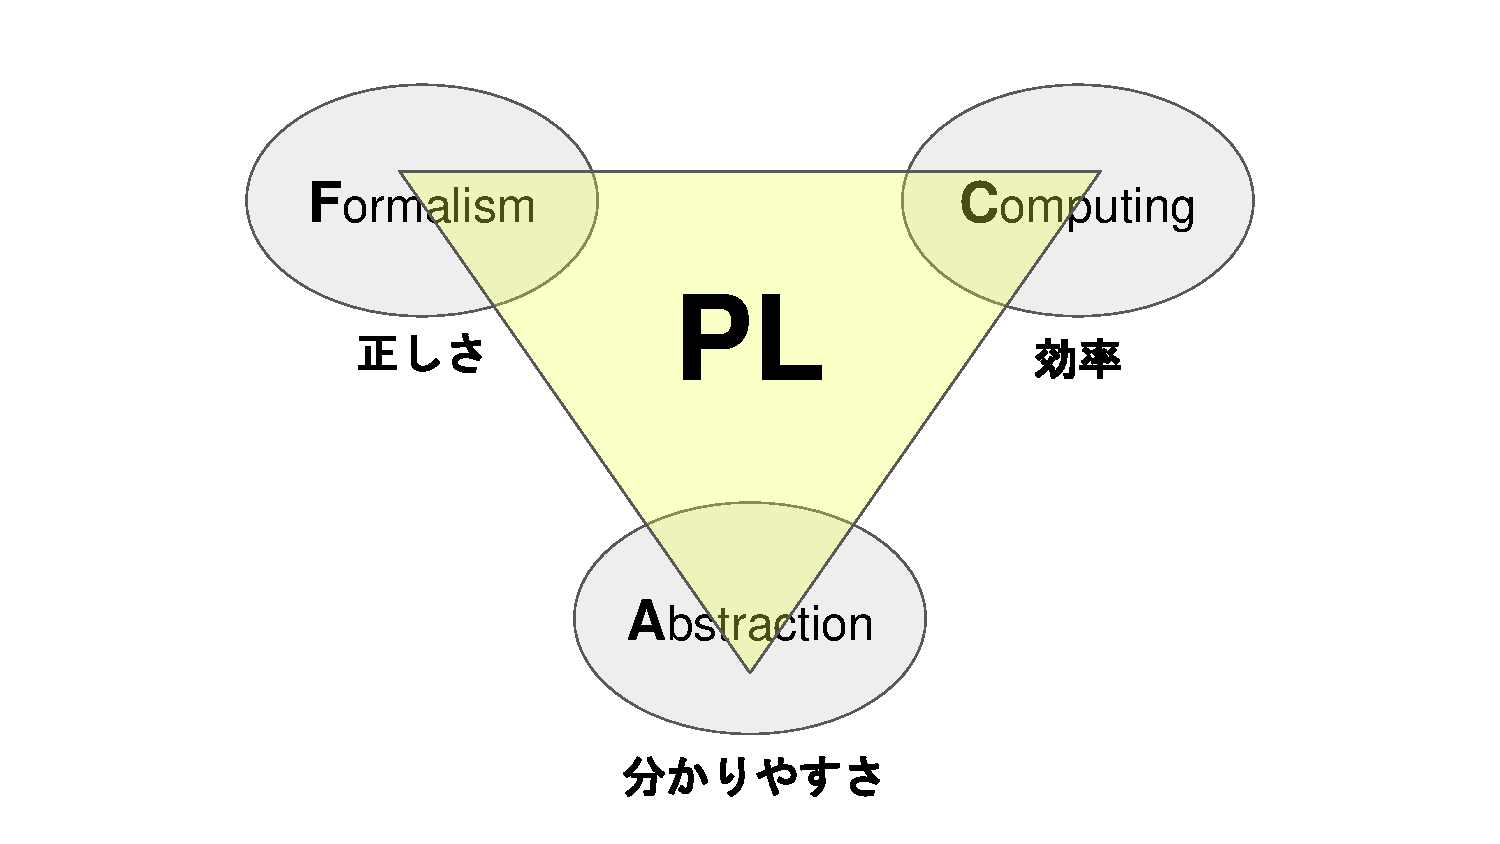
\includegraphics[width=\linewidth,trim=120 20 120 40]{PL-overview.pdf}
 \caption{プログラミング言語(PL)のイメージ}\label{fig:PL-overview}
\end{wrapfigure}
\paragraph{研究の世界観}
プログラミング言語(PL)分野において,実装系の研究に取り組んできている.
私が考えるPL研究のイメージは,右図に示す通り,Computing・Abstraction・
Formalismの3つを橋渡しする枠組みを作ることである.PL分野における実装系と
は,Computingへのウェイトが相対的に大きいという意味でしかないと考えてい
る.これまで,多様なトピックに取り組んできたが,Computing・Abstraction・
Formalismの橋渡しを考えるという点は,常に一貫している.

\paragraph{狭義の専門性}
私がComputingの側面として,特に専門としているのは並列計算である.並列計
算のプログラミングは,簡単な記述・多様な計算・計算機の活用がトリレンマを
成し,全てを成立させるのが困難である.PL的なアプローチ,特に自動並列化や
ドメイン特化言語(DSL)を通じて,この困難に取り組むことに,最も注力して
長期的に取り組んできた.PL実装技術の観点では,コンパイラに関する専門性が
高く,特に自動並列化に関しては,世界に屈指の専門性があると自負している.
過去の研究業績においてもコンパイラや自動並列化に関する仕事(業績
\cite{pldi21:red_par,ipdps21:plex,jip20:centaurus,splash19:nbody,adbis18:par_xpath,jip17:hadoop,aplas14:sd_dfa,pro13:tree_par,pldi11:red_par,aplas09:gpgpu_skel}
)が多く,PL分野のトップ国際会議PLDIで出版されたものもある(業績
\cite{pldi21:red_par,pldi11:red_par}).

\paragraph{研究トピックの広がり}
私の研究のスコープは,並列計算に限ったものではない.先に述べたように,
Computing・Abstraction・Formalismの橋渡しに繋がると考える事柄は,全てス
コープに入る.学生の興味や共同研究者の専門性に合わせて,PL実装に係る様々
なトピックに取り組んできた.例えば,業績
\cite{gpce14:libdsl,aplas16:pyblame,ppl22:plags,pro22o:far_memory,jssst22:checkpoint,splash22:mvnb}
,は,計算の記述(つまりプログラミング)を正しく分かりやすくするためのシ
ステムであり,Computing・Abstraction・Formalismの橋渡しとして機能する.
また,特定のComputing関する事例研究(例えば,業績
\cite{icpp15:htm,ispass21:ib_odp,ppl22:sfa,ispass22:vipp,ppl23c3:otf_sfa})
も重視している.これは,具体的なComputingの事例を分析し,それを定式化・
抽象化することで,地に足のついたPLの成果に繋がると考えているからである.


\section*{個別的な研究内容の概要}
扱う研究のトピックは,大きく分けて,プログラムの変換や解析を扱うコンパイ
ル技術と,プログラミングを支援するライブラリやメモリ管理を扱うランタイム
技術の2つに分類される.

\subsection*{コンパイル技術}

\paragraph{半環に基づく並列化}

 \cite{pldi21:red_par}

 \cite{pldi11:red_par}

 \cite{jssst13:sd_dfa,aplas14:sd_dfa}

 \cite{jip17:hadoop}

 \cite{pro13:tree_par}

\paragraph{代数的性質に基づく効率化}
\cite{splash19:nbody}
\cite{aplas09:gpu_skel}

\paragraph{有限オートマトンに基づく並列化}
\cite{ipdps21:plex,ppl22:sfa,ppl23c3:otf_sfa}
 \cite{ppl23:zdd}

\paragraph{DSL開発支援}

\cite{ppl23c3:satysfi_ted}
\cite{gpce14:libdsl}

\paragraph{プログラム検査・検証}
\cite{ppl21c3:mixed-size_genmc,ppl23c3:mixed-size_genmc}

\cite{ppl22:plags}
\cite{aplas16:pyblame}

\subsection*{ランタイム技術}

\paragraph{木・グラフ処理}

\cite{fhpc16:s6raph,jip21:hyper_gemini}
\cite{ijpp16:tree_skel,jssst16:nbody_locality,jssst14:par_traversal,pro19o:centaurus,jip20:centaurus}
\cite{adbis18:par_xpath,cloudcomp20:xpath}

\cite{ngc18:pregel}
\cite{ispass22:vipp}

\paragraph{並行性制御}
\cite{icpp15:htm,jip22:compth}

\paragraph{リモートメモリアクセス}
\cite{ipdrm20:menps,ispass21:ib_odp,jip22:argodsm,pro22o:far_memory,ppl23c3:far_memory,ppl23c3:redn}

\paragraph{チェックポインティング}
\cite{splash22:mvnb,ppl23:notebook}

\cite{jssst22:checkpoint}


\newpage
\begin{center}
\LARGE\bfseries 今後の研究計画書
\end{center}

\section*{着任後の研究構想}

\subsection*{研究者として}

\paragraph{第一の目標}
私が最も重要だと考えているのは,PL実装研究を続けることである.正確には,
PL実装研究の最前線に身を置き続け,継続的に成果を上げていくことである.も
ちろん,トップ国際会議に採択されるインパクトが大きい成果を上げることも重
要だが,それも持続的な研究が大前提である.そして,PL実装研究は,1本の論
文出版に掛かる労力が膨大であり,1つの研究プロジェクトを完遂させることす
らも大変難しい.

\paragraph{継続の方策}
PL実装研究を教員単独で進めることには限界がある.これは,大学教員の職に就
いてから痛切に感じてきたことである.大きな労力が掛かる実装研究を続ける現
実的な方策は,共同研究の和を広げて,効率的な分業を進めることである.そう
すれば,一人では大きすぎる労力でも対処できる.これは絵空事ではなく,実際
に私と中丸氏との共同研究(業績\cite{splash22:mvnb,ppl23:notebook})において実現した.具体
的には,システムを開発して実験するのが得意な中丸氏が,研究のストーリーを
作って論文を書くのが得意な私と組んで,綿密な連携をとることで,プロジェク
トは驚くほど効率的に進めることができ,複数の論文発表に短時間でこぎつける
ことができた.この共同研究の経験を踏まえて,より広範なトピックについて,
各自が持つ専門性とアドバンテージを適切に組み合わせたチームビルディングを
行うことで,最前線のPL実装研究を続けていこうと考えている.

\paragraph{コンパイラ研究}
チームビルティングや研究マネジメントが,PL実装研究において死活的に重要で
あるが,それに専念しすぎるべきでもないと考えている.特に,自身が持つコン
パイラの専門性は,国内では既に相当稀少なものなってしまった.日本における
コンパイラ研究の芽を絶やさないように,とりわけコンパイラ研究については,
専門性を鈍らせずに筆頭著者としての研究を続けことも目標としている.

\subsection*{研究指導者として}
PIとして研究室を主宰するときには,研究指導者としての役割が死活的に重要で
ある.PL実装研究においてチームビルディングを考えるときに,学生をチームに
入れて研究できなければ,研究グループとして発展しない.しかし,学生は専門
家ではないので,専門家へと育成しながらチームとして研究することが必要にな
る.

助教として学生の研究指導に従事してきた経験から,おおよそ次のようなスケ
ジュールと枠組みで学生に研究指導し,研究のマインドセットを根付かせてから,
緩やかに学生との共同研究を進展させていくのが効果的だと考えている.
\begin{itemize}
 \item 卒業研究は,研究の作法の教育を第一として,追試や事例研究に取り組
       ませて,進学後のM1の前期に論文誌投稿する.

 \item 修士研究は,卒業研究の取り組み方や興味を踏まえて,適性のありそう
       なトピックを割り振る.このとき,当該学生の興味を軸に,他の教員・
       学外研究者との連携も行う.

 \item M2の2月までに,ランク2以上の国際会議に投稿可能な材料を揃えて,3月
       までに論文執筆の主たる作業を終えて,残りの仕事を私が引き取る.

 \item 博士課程への進学は,M1までに少なくとも1本のfull paperを投稿し,M1
       の1月の段階で修士研究に関する進捗を生んでいる学生に対して,意思確
       認の上で,適宜勧める.

 \item 博士研究では,トップ国際会議に挑戦できるような研究テーマとストー
       リーの枠組みを,学生が納得する形で設定し,採択のための方策を指導
       する.

 \item 博士研究では,研究の発展や状況の変化に対して臨機応変に対応する.
       例えば,研究インターンを含めて,本人が取り組んでいるテーマを効率
       良く研究できる環境へと,積極的に送り出す.
\end{itemize}
博士課程の部分については不確定要素が多いが,修士課程までの部分については,
現在指導している博士課程学生(業績
\cite{pro22o:far_memory,jip22:argodsm,ppl23c3:far_memory}の筆頭著者)や
修士修了で企業研究所に就職した学生(業績\cite{ppl22:sfa,ppl23c3:otf_sfa}の筆頭
著者)の反応と成長から,有効性の感触を得ている.この研究指導の枠組みを,
学生の合わせて改良・発展させていくことを考えている.


\newpage
\begin{center}
\LARGE\bfseries 今までの教育経験と教育に関する抱負
\end{center}
\bigskip

\section*{教育関連の実績}

現職,東京大学MIセンター基盤情報部門において,全学的なPythonプログラミン
グ教育に従事している.担当している授業は,「Pythonプログラミング入門」
(以下IPP)と「Pythonプログラミング作法」(以下PPP)である.IPPは,年間
受講者が700人を超える大規模授業であり,PPPは,私が設計して独りで運営して
いる小規模授業(受講生30人程度)である.どちらも,自習を中心としたオンラ
インの反転授業である.

IPPでは着任以降,教材や課題の改訂・保守の業務の大部分を担ってきた.2022
年現在においては,公開オンライン教科書
\footnote{\url{https://utokyo-ipp.github.io/}}の改訂作業は全て私が担って
いる.この教科書の評判はとても良く,東大内に留まらず,Twitter上などで一
般の人からも好評を博し,その品質の高さを称賛されている.

IPPの授業については,2020年度にオンライン授業に移行する段階で,授業設計
に大きく寄与し,現在のオンライン授業の形態を作った.特筆すべき仕事は,課
題演習・採点・講評を助けるWebアプリケーションPLAGS UT(業績
\cite{ppl22:plags})を開発し,授業で運用している点である.PLAGS UTは,
テストコードを使って,課題提出時に自動評価し,即座にフィードバックを返す.
PLAGS UTに基づく自動評価付きの課題演習は,9割以上の受講生から高評価を得
ている.PLAGS UTは,自身が担当するPPPの他,私が担当していない教養学部の
「アルゴリズム入門」においても運用されている.

PLAGS UTの導入は,プログラミング演習授業の生産性を革命的に向上させた.導
入前の2019年は,授業に7名の教員を動員していたが,それよりも受講生が増え
ているにも関わらず,現在は2名で十分足りている.機械的なフィードバックの
おかげで,授業中の質問件数が6割削減され,TAの労働負荷も大幅に改善された.
そして,システムに基づいて体系的なオンライン業務になったことで,TAの満足
度も向上し,リピート希望率は9割近くを達成している.

学部1--2年生向けの「アルゴリズム入門」は,14クラスで開講される完全対面授
業である.非常勤講師を含めた複数の教員が個別にクラスを担当する.このよう
な文脈でも,PLAGS UTは有効に機能し,特に非常勤講師に対して,高品質の課題
演習のパッケージを提供することに役立っている.

以上ような教育DXは,学外でも高く評価された(業績\cite{axies22:plags}).

\section*{着任後の教育構想}

\subsection*{教育に関する抱負}

PLAGS UTの開発と運用のノウハウを活かし,プログラミング教育をシステマチッ
クにしていきたい.システム化を進めることで,特に次の3点が達成できると良
いと考えている.
\begin{itemize}
 \item TAの教育とTAによる教育の促進.

 \item 非常勤講師を活用した教育の品質管理.

 \item 高校の情報教育の変化に応じた迅速なカリキュラム改訂.
\end{itemize}

一方,東大でのPLAGS UTの成功体験を過信しすぎないほうが良いとも考えている.
授業方針や学生の特性は,東大内でも一様ではない.ましてや,別大学である電
通大において,同じ方法論がそのまま使えるとは思わない.しかし,様々な困難
を乗り越えて教育DXを実現するノウハウは確かに獲得した.そのノウハウを獲得
する能力は,電通大での状況を改善することにも役立つと信じている.

\subsection*{授業構想}

\paragraph{言語処理系(学部)}
\begin{itemize}
 \item インタプリタ
 \item 部分評価
 \item 埋め込み言語
\end{itemize}

\paragraph{ソフトウェア工学(学部)}
\begin{itemize}
 \item GitHub
 \item テスト
 \item 形式手法
\end{itemize}

\paragraph{プログラム言語基礎論(大学院)}
\begin{itemize}
 \item 操作的意味論
 \item 型システム
 \item ラムダ計算
\end{itemize}

\newpage
\begin{center}
\LARGE\bfseries 応募者に関する参考意見を伺える方
\end{center}
\bigskip

\section*{名簿}
\begin{center}
\begin{tabular}[t]{llllll}
氏名 & 所属 & 職位 & Emailアドレス \\ \hline
千葉滋 & 東京大学 & 教授 & \url{chiba@chibas.net}  \\
田浦健次朗 & 東京大学 & 教授$^\dagger$ & \url{tau@eidos.ic.i.u-tokyo.ac.jp} \\
Zhenjiang Hu & Peking University & Professor$^\ddagger$ & \url{huzj@pku.edu.cn} \\
\end{tabular}
\medskip\\
\noindent
$^\dagger$ 情報基盤センター長
\qquad
\noindent
$^\ddagger$ Dean of School of Computer Science
\end{center}
\paragraph{連絡先住所(居室)}
\begin{center}
\begin{tabular}[t]{ll}
千葉滋 & 〒113-8656 東京都文京区本郷7-3-1 東京大学 情報理工学系研究科創造情報学専攻 \\
田浦健次朗 & 〒113-0033 東京都文京区本郷7-3-1 東京大学 工学部2号館10F101D2号室 \\
Zhenjiang Hu & Room 1247, Science Building \#1, Peking University \\
\end{tabular}
\end{center}

\section*{応募者との関係}
\paragraph{千葉滋}
私が所属する所属MIセンター基盤情報部門の部門長であり,直属の上司.千葉先
生は,学内の情報教育に関する情報交換を行う委員会である情報教育ネットワー
クの取りまとめ役を務めており,私はその補佐を行っている.形式上は,研究指
導や授業運営を共同したことはないが,私が獲得したACT-Iの予算における研究
アドバイザーを務めており,私の専門性は十分理解している.また,MIセンター
業務としてPLAGS UTを開発運用している様子は,駒場の「アルゴリズム入門」の
担当教員の立場で見てきている.したがって,私の研究と教育の実務を把握し,
評価できる人物である.

\paragraph{田浦健次朗}
私が研究業務を行うために所属している田浦研究室の長であり,MIセンター基盤
情報部門を兼担している.2015年度にポスドクとして田浦研究室に所属した際は,
CRESTのプロジェクトでN体ソルバに関する研究に従事した.その縁から,MIセン
ターの助教に着任するときに,田浦研究室に所属して研究を行うことになった.
田浦研究室では,田浦先生と共同して学生の研究指導に当たっている.私を研究
者及び研究指導者として評価できる人物である.

\paragraph{Zhenjiang Hu}
私が学生時代から研究上お世話になっている人物である.私はB4のときから,東
大計数数理の武市研究室に訪問しており,そこで武市先生とHu先生のお世話になっ
た.また,武市先生が退官して武市研究室が解散した後は,NIIのHu研究室に訪
問して研究するようになった.Hu先生が北京大に移動した後は,会う頻度こそ減っ
たものの,未だに私の専門に近いトピックを扱い続けており,私の研究内容や研
究活動について客観的に評価できる人物である.

\newpage
\begin{thebibliography}{100}
 %% Journal (refereed)
 \bibitem{jip22:argodsm} Hideshima, T., Sato, S., and Taura, K. 2022. Cost-aware Programming on Page-based Distributed Shared Memory. J. Inf. Process., 30:463–475.
 \bibitem{jip22:compth} Endo, W., Sato, S., and Taura, K. 2022. ComposableThreads: Rethinking User-level Threads with Composability and Parametricity in C++. J. Inf. Process., 30:269–282. (Specially Selected Paper)
 \bibitem{jip21:hyper_gemini} Fujimura, S., Sato, S., and Taura, K. 2021. An Efficient and Scalable Distributed Hypergraph Processing System. J. Inf. Process., 29:812–822.
 \bibitem{jip20:centaurus} Sato, S., Ihara, H., and Taura, K. 2020. CENTAURUS: A Dynamic Parser Generator for Parallel Ad Hoc Data Extraction. J. Inf. Process., 28:724–732.
 \bibitem{ngc18:pregel} Sato, S. 2018. On Implementing the Push-Relabel Algorithm on top of Pregel. New Gener. Comput., 36(4):419–449.
 \bibitem{jip17:hadoop} Miyazaki, R., Matsuzaki, K., and Sato, S. 2017. A Generator of Hadoop MapReduce Programs that Manipulate One-dimensional Arrays. J. Inf. Process., 25:841–851.
 \bibitem{ijpp16:tree_skel} Sato, S. and Matsuzaki, K. 2016. A Generic Implementation of Tree Skeletons. Int. J. Parallel Program., 44(3):686–707.
 \bibitem{compsoft15:takano} 高野保真,岩崎英哉,佐藤重幸.2015.Glasgow Haskell Compiler上の遅延オブジェクト再利用手法の設計と実装.コンピュータソフトウェア,32(1):253–287.
 \bibitem{pro13:tree_par} 佐藤重幸,松崎公紀.2013.木上のスケルトン並列プログラミングのための演算子生成器.情報処理学会論文誌プログラミング(PRO),6(4):38–49.

 %% Conference proceedings (refereed)
 \bibitem{pldi21:red_par} Morihata, A. and Sato, S. 2021. Reverse Engineering for Reduction Parallelization via Semiring Polynomials. In Proc. the 42nd ACM SIGPLAN Conference on Programming Language Design and Implementation (PLDI 2021), pp.820–834.
 \bibitem{ipdps21:plex} Li, L., Sato, S., Liu, Q., and Taura, K. 2021. Plex: Scaling Parallel Lexing with Backtrack-Free Prescanning. In Proc. the 35th IEEE International Parallel and Distributed Processing Symposium (IPDPS 2021), pp.693–702.
 \bibitem{ispass21:ib_odp} Fukuoka, T., Sato, S., and Taura, K. 2021. Pitfalls of InfiniBand with On-Demand Paging. In Proc. 2021 IEEE International Symposium on Performance Analysis of Systems and Software (ISPASS 2021), pp.265–275.
 \bibitem{ipdrm20:menps} Endo, W., Sato, S., and Taura, K. 2020. MENPS: A Decentralized Distributed Shared Memory Exploiting RDMA. In Proc. the 4th IEEE/ACM Annual Workshop on Emerging Parallel and Distributed Runtime Systems and Middleware (IPDRM 2020), pp.9–16.
 \bibitem{adbis18:par_xpath} Sato, S., Hao, W., Matsuzaki, K. 2018. Parallelization of XPath Queries using Modern XQuery Processors. In Proc. the 22nd European Conference on Advances in Databases and Information Systems (ADBIS 2018), Short Paper, pp.54–62.
 \bibitem{aplas16:pyblame} Arai, R., Sato, S., and Iwasaki, H. 2016. A Debugger-Cooperative Higher-Order Contract System in Python. In Proc. the 14th Asian Symposium on Programming Languages and Systems (APLAS 2016), pp.148–168.
 \bibitem{fhpc16:s6raph} Coll Ruiz, O., Matsuzaki, K., and Sato, S. 2016. s6raph: Vertex-Centric Graph Processing Framework with Functional Interface. In Proc. Proceedings of the 5th International Workshop on Functional High-Performance Computing (FHPC 2016), pp.58–64.
 \bibitem{icpp15:htm} Kobayashi, T., Sato, S., and Iwasaki, H. 2015. Efficient Use of Hardware Transactional Memory for Parallel Mesh Generation. In Proc. the 44th International Conference on Parallel Processing (ICPP 2015), pp.600–609.
 \bibitem{gpce14:libdsl} Shioda, M., Iwasaki, H., and Sato, S. 2014. LibDSL: A Library for Developing Embedded Domain Specific Languages in D via Template Metaprogramming. In Proc. the 13th International Conference on Generative Programming: Concepts and Experiences (GPCE 2014), pp.63–72.
 \bibitem{aplas14:sd_dfa} Sato, S. and Morihata, A. 2014. Syntax-Directed Divide-and-Conquer Data-Flow Analysis. In Proc. the 12th Asian Symposium on Programming Languages and Systems (APLAS 2014), pp.392–407.
 \bibitem{pldi11:red_par} Sato, S. and Iwasaki, H. 2011. Automatic Parallelization via Matrix Multiplication. In Proc. the 32nd ACM SIGPLAN conference on Programming Language Design and Implementation (PLDI 2011), pp.470–479.
 \bibitem{aplas09:gpu_skel} Sato, S. and Iwasaki, H. 2009. A Skeletal Parallel Framework with Fusion Optimizer for GPGPU Programming. In Proc. the 7th Asian Symposium on Programming Languages and Systems (APLAS 2009), pp.79–94.

 %% Conference proceedings (non-refereed)
 \bibitem{splash22:mvnb} Nakamaru, T. and Sato, S. 2022. Multiverse Notebook: A Notebook Environment for Safe and Efficient Exploration. In Proc. the 2022 ACM SIGPLAN International Conference on Systems, Programming, Languages, and Applications: Software for Humanity (SPLASH Companion 2022), pp.7–8. (Extended Poster Abstract)
 \bibitem{ispass22:vipp} Sato, S., Iizuka, K., Yoshifuji, N., and Natsume, M. 2022. VIPP: Validation-Included Precision-Parametric N-Body Benchmark Suite. In Proc. 2022 IEEE International Symposium on Performance Analysis of Systems and Software (ISPASS 2022), pp.156–158. (Extended Poster Abstract)
 \bibitem{cloudcomp20:xpath} Hao, W., Matsuzaki, K., and Sato, S. 2021. A Dual-Index Based Representation for Processing XPath Queries on Very Large XML Documents. In Proc. the 10th EAI International Conference on Cloud Computing (CloudComp 2020), pp.18–30.
 \bibitem{splash19:nbody} Sato, S. 2019. A Symmetry-Based N-Body Solver Compiler. In Proc. the 2019 ACM SIGPLAN International Conference on Systems, Programming, Languages, and Applications: Software for Humanity (SPLASH Companion 2019), pp.21–22. (Extended Poster Abstract)

 %% Overview, Review
 \bibitem{ieice19:python} 佐藤重幸.2019.データ処理のためのプログラミング言語[V・完]―Python 言語編―.電子情報通信学会誌, 102(12):1135–1139

 %% Oral presentation (unpublished)
 \bibitem{ppl23:zdd} 佐藤重幸.2023.ZDDによる並列正規表現マッチング.第25回プログラミングおよびプログラミング言語ワークショップ(PPL 2023)カテゴリ1.
 \bibitem{ppl23:notebook} 中丸智貴,佐藤重幸.2023.ノートブックプログラミングにおける手戻りの調査と分析.第25回プログラミングおよびプログラミング言語ワークショップ(PPL 2023)カテゴリ1.
 \bibitem{jssst22:checkpoint} 中田昌輝,鵜川始陽,佐藤重幸.2022.プログラムを停止させない定期的な不揮発性メモリへのチェックポインティング.日本ソフトウェア科学会第 39 回大会. (筆頭著者が優秀発表賞を受賞)
 \bibitem{pro22o:far_memory} 秀島宇音,佐藤重幸,田浦健次朗.2022.C++におけるポインタベースのデータ構造のためのFar Memoryアロケータ.第140回プログラミング研究発表会.
 \bibitem{ppl22:sfa} 高品剛大,佐藤重幸,田浦健次朗.2022.Simultaneous Finite Automatonの部分構成による並列正規表現マッチ.第24回プログラミングおよびプログラミング言語ワークショップ(PPL 2022)カテゴリ1.
 \bibitem{ppl22:plags} 佐藤重幸,犬伏貴之.2022.PLAGS UT: 自動評価付きPythonプログラミング課題管理システム.第24回プログラミングおよびプログラミング言語ワークショップ (PPL 2022)カテゴリ1.
 \bibitem{pro19o:centaurus} Sato, S., Ihara, H., and Taura, K. 2019. Centaurus: A Just-in-time Parallel-parser Generator for Ad Hoc Data Processing. 第125回プログラミング研究発表会.(山下記念研究賞)
 \bibitem{jssst16:nbody_locality} 佐藤重幸,田浦健次朗.2016.一般化N体問題アルゴリズムに対する局所性向上技法.日本ソフトウェア科学会第33回大会.(高橋奨励賞)
 \bibitem{jssst14:par_traversal} 佐藤重幸. 2014.局所性を意識した並列反復木走査.日本ソフトウェア科学会第31回大会.(優秀発表賞)
 \bibitem{jssst13:sd_dfa} 佐藤重幸,森畑明昌.2013.構文主導型データフロー解析の並列実装.日本ソフトウェア科学会第30回大会.(優秀発表賞)

 %% Poster presentation (unpublished)
 \bibitem{ppl23c3:redn} 利根悠司,佐藤重幸,田浦健次朗.2023.自己書き換え的な InfiniBand Verbs コードを生成するEDSL.第25回プログラミングおよびプログラミング言語ワークショップ(PPL 2023)カテゴリ3.
 \bibitem{ppl23c3:far_memory} 秀島宇音,佐藤重幸,田浦 健次朗.2023.C++におけるfar-memoryデータ構造のためのアロケータ抽象化.第25回プログラミングおよびプログラミング言語ワークショップ(PPL 2023)カテゴリ3.
 \bibitem{ppl23c3:otf_sfa} 高品剛大,佐藤重幸,田浦健次朗.2023.On-the-fly Simultaneous Finite Automatonによる並列正規表現マッチング.第25回プログラミングおよびプログラミング言語ワークショップ(PPL 2023)カテゴリ3.
 \bibitem{ppl23c3:satysfi_ted} 小林亮太,佐藤重幸,田浦健次朗.2023.SATySFi におけるドメイン固有型エラー診断.第25回プログラミングおよびプログラミング言語ワークショップ(PPL 2023)カテゴリ3.
 \bibitem{ppl23c3:mixed-size_genmc} 水橋大瑶,佐藤重幸,田浦健次朗.2023.Mixed-Size Accessesを含む並行Cプログラムの効率的なステートレスモデル検査.第25回プログラミングおよびプログラミング言語ワークショップ(PPL 2023)カテゴリ3.
 \bibitem{ppl21c3:mixed-size_genmc} 木村元紀,佐藤重幸,田浦健次朗.2022.混合サイズアクセスのある並行Cプログラム向けモデル検査器.第24回プログラミングおよびプログラミング言語ワークショップ(PPL 2022)カテゴリ3.

 %% Invited talk (unpublished)
 \bibitem{axies22:plags} 佐藤重幸.2022.PLAGS UT: 自動評価付き Python プログラミング課題管理システム.大学ICT推進協議会 2022年度年次大会OSS企画セッション.

 %% Misc
 \bibitem{compsoft19:phd_course} 佐藤重幸.2019.(情報系)博士課程進学とその先.コンピュータソフトウェア, 36(1):85–87.
 \bibitem{ipsj19:pldi2016} 佐藤重幸.2016.PLDI 2016報告.情報処理学会 会誌 57(11):1154–1156.
 \bibitem{compsoft16:pldi2015} 佐藤重幸.2016.PLDI 2015報告.コンピュータソフトウェア,33(1):15–21.
\end{thebibliography}
\end{document}

